\documentclass{beamer}
\usepackage[euler-digits]{eulervm}
\usepackage{tikz}
\usefonttheme{professionalfonts}
\mode<presentation>
%%%%%%%%%%%%%%%%%%%%%%%%%%%%%%%%%%%%%%%%%%%%%%%%%%%%%%%%%%%%%%%%%%%%%%%%%%%%%%%
\title{Evaluation of the Mittag-Leffler Function}
\author{William McLean}
\date{9 June, 2020}
\begin{document}
%%%%%%%%%%%%%%%%%%%%%%%%%%%%%%%%%%%%%%%%%%%%%%%%%%%%%%%%%%%%%%%%%%%%%%%%%%%%%%%
\begin{frame}
\titlepage
\end{frame}
\begin{frame}{Outline}
\tableofcontents
\end{frame}
%%%%%%%%%%%%%%%%%%%%%%%%%%%%%%%%%%%%%%%%%%%%%%%%%%%%%%%%%%%%%%%%%%%%%%%%%%%%%%%
\section{Background}
\begin{frame}{Background}
\begin{quote}
In recent times the attention of mathematicians and applied scientists towards 
the functions of Mittag-Leffler type has increased, overall because of their 
relation to the fractional calculus and its applications. Because the 
fractional calculus has attracted wide interest in different areas of applied 
sciences, we think that the Mittag-Leffler function is now beginning to leave  
behind its isolated life as Cinderella. 
\end{quote}

Gorenflo, Kilbas, Mainardi and Rogosin, \emph{Mittag-Leffler Functions, 
Related Topics and Applications}, Springer, 2014. 
\end{frame}

\begin{frame}
\begin{itemize}
\item Gorenflo, Loutchko and Luchko, 
\href{http://citeseerx.ist.psu.edu/viewdoc/summary?doi=10.1.1.501.3682}%
{Computation of the Mittag-Leffler function $E_{\alpha,\beta}(z)$ and its 
derivatives}, \emph{FCAA}, 2002.
\item Weideman and Trefethen, 
\href{https://www.ams.org/journals/mcom/2007-76-259/S0025-5718-07-01945-X/}%
{Parabolic and hyperbolic contours for computing the Bromwich integral},
\emph{Math. Comp.}, 2007.
\item Seybold and Hilfer, 
\href{https://epubs.siam.org/doi/10.1137/070700280}%
{Numerical algorithm for calculating the generalized Mittag-Leffler function},
\emph{SINUM}, 2008.
\item Garrappa and Popolizio, 
\href{https://link.springer.com/article/10.1007/s10444-012-9274-z}%
{Evaluation of generalized Mittag-Leffler functions on the real line},
\emph{Adv. Comput. Math.}, 2013.
\item Gill and Straka, 
\href{https://strakaps.github.io/MittagLeffleR/}%
{MittagLeffleR: Using the Mittag-Leffler distributions in R}, 2017.
\item  Igor Podlubny,
\href{https://www.mathworks.com/matlabcentral/fileexchange/%
8738-mittag-leffler-function}%
{Mittag-Leffler function}, MATLAB Central File Exchange, 2012--2020. 
\end{itemize}
\end{frame}
\begin{frame}{Origin}
In 1902, Mittag-Leffler considered the problem of analytic continuation of a
power series
\[
FC(z)=k_0+k_1z+k_2z^2+\cdots
\]
assuming
\[
\lim_{n\to\infty}|k_n|^{1/n}=\frac{1}{r}<\infty
\quad\text{(so $r=\text{radius of convergence}$).}
\]
He associated with $FC(z)$ the entire function
\[
F_\alpha(z)=k_0+\frac{k_1z}{\Gamma(1+\alpha)}+\frac{k_2z^2}{\Gamma(1+2\alpha)}
    +\cdots=\sum_{n=0}^\infty\frac{k_nz^n}{\Gamma(1+n\alpha)}
\]
for $0<\alpha\le1$.  (Abel had previously considered $F_1(z)$.)
\end{frame}
\begin{frame}
Mittag-Leffler obtained the representation
\[
FA(z)=\lim_{\alpha\to1}\int_0^\infty 
    e^{-\omega}F_\alpha(\omega^\alpha z)\,d\omega
\]
for the analytic continuation of the power series~$FC(z)$, and was led to study 
the special case~$k_n=1$, which he denoted
\[
E_\alpha(z)=\sum_{n=0}^\infty\frac{z^n}{\Gamma(1+n\alpha)}.
\]
Notice
\[
E_0(z)=\frac{1}{1-z}\quad\text{and}\quad
E_1(z)=e^z.
\]
Can show
\[
E_{1/2}(z)=\operatorname{erfcx}(-z)=\exp(z^2)\operatorname{erfc}(-z).
\]
\end{frame}
\begin{frame}
\begin{center}
\includegraphics[scale=0.6]{E_plots.pdf}
\end{center}
\end{frame}
\begin{frame}{Application: fractional relaxation equation}
The fractional IVP
\[
\partial_t u+\lambda\partial_t^{1-\alpha}u=0
    \quad\text{for $t>0$, with $u(0)=u_0$,}
\]
is given by $u(t)=u_0 E_\alpha(-\lambda t^\alpha)$.
\vfill
Here, the Riemann--Liouville fractional derivative of order~$\mu$ is defined 
by
\[
(\partial_t^\mu u)(t)=\partial_t(\mathcal{I}^{1-\mu}u)(t),\quad0<\mu<1,
\]
and the fractional integral by
\[
(\mathcal{I}^\mu u)(t)=\frac{1}{\Gamma(\mu)}\int_0^t(t-s)^{\mu-1}u(s)\,ds,
\quad\mu>0.
\]
\end{frame}

\begin{frame}{Application: Mittag-Leffler distribution}
A random variable~$X$ has a Mittag-Leffler probability distribution if
\[
P(X<x)=1-E_\alpha(-x^\alpha),\quad x>0.
\]
We will see shortly that 
\[
\mathcal{L}\{E_\alpha(-x^\alpha)\}=\int_0^\infty 
    e^{-\lambda x}E_\alpha(-x^\alpha)\,dx=\frac{1}{\lambda+\lambda^{1-\alpha}},
\]
and therefore the Laplace transform of the probability density function~$p(x)$ 
is
\[
\mathbb{E}(e^{-\lambda X})=\lambda\mathcal{L}\{1-E_\alpha(-x^\alpha)\}
    =\frac{1}{1+\lambda^\alpha}
\]
The Mittag-Leffler density is heavy tailed:
\[
p(x)=O(x^{-\alpha-1})\quad\text{as $x\to\infty$.}
\]
\end{frame}

\begin{frame}{Gamma function and Hankel contour}
\[
\frac{1}{\Gamma(1+n\alpha)}=\frac{1}{2\pi i}\int_{\mathcal{C}}
    \frac{e^w}{w^{1+n\alpha}}\,dw.
\]
\vfill
\begin{center}
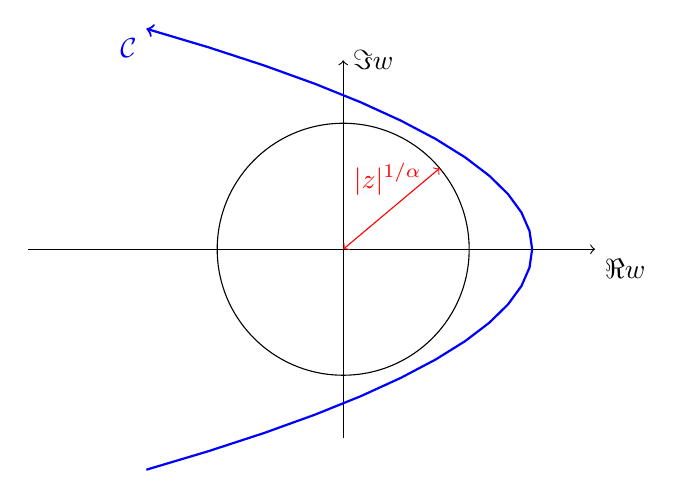
\begin{tikzpicture}[scale=0.8]
\draw[->] (-5,0) -- (4,0);
\node[below right] at (4,0) {$\Re w$};
\draw[->] (0,-3) -- (0,3);
\node[right] at (0,3) {$\Im w$};
\draw[->,thick,domain=-3.5:3.5, blue] plot (3-\x*\x/2, \x);
\draw[-] (0, 0) circle [radius=2];
\node[blue, below left] at ({-25/8}, 3.5) {$\mathcal{C}$};
\draw[<->,red] (0,0) -- ({2*cos(40)}, {2*sin(40)});
\node[red,above] at ({sqrt(2)/2},{sqrt(2)/2}) {$|z|^{1/\alpha}$};
\end{tikzpicture}
\end{center}
\end{frame}
\begin{frame}{Integral representation}
Given $z\in\mathbb{C}$, choose $\mathcal{C}$ passing to the right of the
disk~$|w|<|z|^{1/\alpha}$, so that $|z/w^\alpha|<1$ for all 
$w\in\mathcal{C}$ and hence
\begin{align*}
E_\alpha(z)&=\sum_{n=0}^\infty\frac{z^n}{\alert{\Gamma(1+n\alpha)}}
    =\sum_{n=0}^\infty\frac{z^n}{\alert{2\pi i}}\alert{\int_{\mathcal{C}}
	\frac{e^w\,dw}{w^{1+n\alpha}}}\\
	&=\frac{1}{2\pi i}\int_{\mathcal{C}}\frac{e^w}{w}\sum_{n=0}^\infty
	\biggl(\frac{z}{w^\alpha}\biggr)^n\,dw\\
	&=\frac{1}{2\pi i}\int_{\mathcal{C}}
	\frac{e^w}{w}\,\frac{dw}{1-zw^{-\alpha}}.
\end{align*}
Remark: substitution $w=\lambda x$ gives
\[
E_\alpha(-x^\alpha)=\frac{1}{2\pi i}\int_{\mathcal{C}}
    \frac{e^{\lambda x}\,d\lambda}{\lambda+\lambda^{1-\alpha}}
    =\mathcal{L}^{-1}\biggl\{\frac{1}{\lambda+\lambda^{1-\alpha}}\biggr\}.
\]
\end{frame}
\begin{frame}{Asymptotic Behaviour}
Restrict our attention to the case~$z=-x$ for~$x>0$, and write
\[
E_\alpha(-x)=\frac{1}{2\pi i}\int_{\mathcal{C}}e^wF(w,x)\,dw 
\]
where
\[
F(w,x)=\frac{1}{w}\,\frac{1}{1+xw^{-\alpha}}
    =\frac{w^{\alpha-1}}{x}\,\frac{1}{1+x^{-1}w^\alpha}.
\]
To see how $E_\alpha(-x)$ behaves as~$x\to\infty$, use the identity
\[
\frac{1}{1+x^{-1}w^\alpha}=\sum_{k=0}^{N-1}(-x^{-1}w^\alpha)^k
    +\frac{(-x^{-1}w^\alpha)^N}{1+x^{-1}w^\alpha}
\]
to obtain
\[
E_\alpha(-x)=\sum_{k=0}^{N-1}\frac{1}{2\pi i}\int_{\mathcal{C}}
    e^w\,\frac{w^{\alpha-1}}{x}\,(-x^{-1}w^\alpha)^k\,dw+R_N(x).
\]
\end{frame}
\begin{frame}
Putting $n=k+1$,
\begin{align*}
\sum_{k=0}^{N-1}&\frac{1}{2\pi i}\int_{\mathcal{C}}
    e^w\,\frac{w^{\alpha-1}}{x}\,(-x^{-1}w^\alpha)^k\,dw\\
    &=\sum_{n=1}^N\frac{(-1)^{n-1}x^{-n}}{\alert{2\pi i}} 
    \alert{\int_{\mathcal{C}}\frac{e^w\,dw}{w^{1-n\alpha}}}
\end{align*}    
and thus
\[
E_\alpha(-x)=\sum_{n=1}^N\frac{(-1)^{n-1}x^{-n}}{\alert{\Gamma(1-n\alpha)}}
    +R_N(x)\quad\text{as $x\to\infty$.}
\]
\vfill
\begin{itemize}
\item R.~B.~Paris, Asymptotics of the Mittag-Leffler function $E_a(z)$
on the negative real axis when $a\to1$, arXiv, 2020.
\end{itemize}
\end{frame}
%%%%%%%%%%%%%%%%%%%%%%%%%%%%%%%%%%%%%%%%%%%%%%%%%%%%%%%%%%%%%%%%%%%%%%%%%%%%%%%
\section{Evaluation by Quadrature}
\begin{frame}{Evaluation by Quadrature}
Choose a Hankel contour~$\mathcal{C}$ of the form
\[
w(u)=\mu\bigl(1+\sin(iu-\phi)\bigr),\quad-\infty<u<\infty,
\]
with $\mu>0$ and $0<\phi<\pi/2$.  Since
\begin{align*}
\Re w&=\mu(1-\cosh u\,\sin\phi),\\
\Im w&=\mu\sinh u\,\cos\phi,
\end{align*}
we see that
\[
\Re w(u)\approx-(\tfrac12\mu\sin\phi)e^{|u|}\quad\text{for large $|u|$,}
\]
so $e^{w(u)}$ exhibits a double exponential decay as~$|u|\to\infty$.
\vfill
Find $\mathcal{C}$ is the left branch of the hyperbola with asymptotes
\[
\Im w=\pm(\Re w-1)\cot\phi.
\]
\end{frame}
\begin{frame}
Recall
\[
F(w,x)=\frac{1}{w}\,\frac{1}{1+xw^{-\alpha}}=\frac{w^{\alpha-1}}{w^\alpha+x}
\]
and
\[
E_\alpha(-x)=\frac{1}{2\pi i}\int_{\mathcal{C}}e^wF(w,x)\,dw.
\]
Put
\[
G(u,x)=F\bigl(w(u),x\bigr)w'(u)
\]
so
\[
E_\alpha(-x)=\frac{1}{2\pi i}\int_{-\infty}^\infty e^{w(u)}G(u,x)\,du
\approx Q_h(x),
\]
where, for a step-size~$h>0$,
\[
Q_h(x)=\frac{h}{2\pi i}\sum_{n=-\infty}^\infty e^{w(nh)}G(nh,x).
\]
\end{frame}
\begin{frame}
\begin{center}
\pgfmathsetmacro{\rval}{0.6}
\pgfmathsetmacro{\sval}{0.7}
\pgfmathsetmacro{\phival}{0.8}
\begin{tikzpicture}[scale=1.1]
\draw[->,thick] (-2,0) -- (2,0);
\node[right] at (2,0) {$u$};
\draw[->] (0,-2) -- (0,2);
\node[above] at (0,2) {$v$};
\draw[->,blue] (-2,\rval) -- (2,\rval);
\node[above,blue] at (1,\rval) {$v=r$};
\draw[->,red] (-2,-\sval) -- (2,-\sval);
\node[above,red] at (1,-\sval) {$v=-s$};
\draw[-] (-0.1,-\phival) -- (0.1,-\phival);
\node[left] at (-0.1,-\phival) {$-\phi$};
\draw[-] (-0.1,1.57) -- (0.1,1.57);
\node[left] at (-0.1,1.57) {$\pi/2$};
\end{tikzpicture}
\pgfmathsetmacro{\phideg}{deg(\phival)}
\pgfmathsetmacro{\phipr}{deg(\phival+\rval)}
\pgfmathsetmacro{\phims}{deg(\phival-\sval)}
\hfill
\begin{tikzpicture}[scale=1.1]
\draw[->] (-2,0) -- (1.5,0);
\node[right] at (1.5,0) {$\Re w$};
\draw[->] (0,-2) -- (0,2);
\node[above] at (0,2) {$\Im w$};
\draw[-] (1,-0.1) -- (1,0.1);
\node[below right] at (1,0) {$1$};
\draw[->,domain=-1.7:1.7,blue] plot 
    ({1-sin(\phipr)*cosh(\x)},{cos(\phipr)*sinh(\x)});
\draw[->,thick,domain=-1.7:1.7] plot 
    ({1-sin(\phideg)*cosh(\x)},{cos(\phideg)*sinh(\x)});
\draw[->,domain=-1.4:1.4,red] plot 
    ({1-sin(\phims)*cosh(\x)},{cos(\phims)*sinh(\x)});
\draw[-,dashed] (1,0) -- ({1-2*tan(\phideg)},2);
\draw[-] (0,{0.4+cot(\phideg)}) arc 
    [radius=0.4, start angle=90, end angle={90+\phideg}];
\node[above left] at (0,{0.3+cot(\phideg)}) {$\phi$};
\end{tikzpicture}
\end{center}
\vfill
\[
w(u+iv)=\mu\Bigl(1+sin\bigl(iu-(\phi+v)\bigr)\Bigr).
\]
\end{frame}
\begin{frame}{Quadrature error}
For $0<\phi+v<\pi/2$, put
\[
M(x,v)=\frac{1}{2\pi}\int_{-\infty}^\infty\bigl|e^{w(u+iv)}G(u+iv,x)\bigr|\,du.
\]
It can be shown using contour integration that
\[
\bigl|Q_h(x)-E_\alpha(-x)\bigr|\le\frac{M(x,r)}{\exp(2\pi r/h)-1}
	+\frac{M(x,-s)}{\exp(2\pi s/h)-1}.
\]
In practice, we compute only a finite sum,
\[
Q_{h,N}(x)=\frac{h}{2\pi i}\sum_{n=-N}^N e^{w(nh)}G(nh,x),
\]
resulting in an additional truncation error
\[
\frac{h}{2\pi i}\sum_{|n|\ge N+1}^\infty e^{w(nh)}G(nh,x).
\]
\end{frame}
\begin{frame}{Heuristic error bound}
For $-\infty<u<\infty$,
\begin{align*}
\Re w(u+ir)&\le\mu\bigl(1-\sin(\phi+r)\bigr),\\
\Re w(u-is)&\le\mu\bigl(1-\sin(\phi-s)\bigr),
\end{align*}
so, for the extremal values $r^\star=\pi/2-\phi$ and $s^\star=\phi$, 
\[
M(x,r^\star)=O(1)\quad\text{and}\quad M(x,-s^\star)=O\bigl(\exp(\mu)\bigr).
\]
Likewise,
\[
\Re w(nh)\le\mu\bigl(1-\sin\phi\,\cosh(Nh)\bigr)
\quad\text{for $|n|\ge N+1$,}
\]
so
\begin{multline*}
E_\alpha(-x)=Q_{h,N}(x)+O\Bigl(\exp(-2\pi r^\star/h)\\
	+\exp(\mu-2\pi s^\star/h)
	+\exp\bigl(\mu(1-\sin\phi\,\cosh(Nh)\bigr)\Bigr).
\end{multline*}
\end{frame}
\begin{frame}{Optimal parameters}
Strategy: balance the three error terms by ensuring
\[
-\frac{2\pi r^\star}{h}=\mu-\frac{2\pi s^\star}{h}
	=\mu\bigl(1-\sin\phi\,\cosh(Nh)\bigr).
\]
The left-hand equation implies
\[
\mu=\frac{2\pi(s^\star-r^\star)}{h}=\frac{\pi(4\phi-\pi)}{h}
\]
and then the right-hand equation implies
\[
\cosh(Nh)=\frac{2\phi}{(4\phi-\pi)\sin\phi}
\quad\text{with}\quad\frac{\pi}{4}<\phi<\frac{\pi}{2}.
\]
Thus,
\[
Nh=A(\phi)\equiv\operatorname{arcosh}\biggl(
	\frac{2\phi}{(4\phi-\pi)\sin\phi}\biggr).
\]
\end{frame}
\begin{frame}
We see that
\[
h=\frac{A(\phi)}{N}\quad\text{and}\quad
\mu=\frac{\pi(4\phi-\pi)}{A(\phi)}\,N,
\]
with
\[
-\frac{2\pi r^\star}{h}=\mu-\frac{2\pi s^\star}{h}
	=\mu\bigl(1-\sin\phi\,\cosh(Nh)\bigr)=-B(\phi)N,
\]
where
\[
B(\phi)=\frac{\pi(\pi-2\phi)}{A(\phi)}.
\]
Consequently,
\[
E_\alpha(-x)=Q_{h,N}(x)+O\bigl(e^{-B(\phi)N}\bigr)
\]
\end{frame}
\begin{frame}{Maximise $B(\phi)$}
\[
\max_{\pi/4<\phi<\pi/2}B(\phi)=B(\phi^\star)=2{\cdot}31565\,40324\,80739
\]
\vfill
\begin{center}
\includegraphics[scale=0.5]{../notes/Bplot.pdf}
\end{center}
\end{frame}
\begin{frame}
With $\phi=\phi^\star=1{\cdot}17210$, we find
\[
h=\frac{A(\phi^\star)}{N}=\frac{1{\cdot}08179}{N}
\]
and
\[
\mu=\frac{\pi(4\phi^\star-\pi)}{A(\phi^\star)}\,N=4{\cdot}49208\,N.
\]
Hence,
\[
e^{-B(\phi^\star)N}=\frac{1}{10.1315^N}.
\]
\end{frame}
\begin{frame}{The points $w(nh)$ for $0\le n\le N$}
\begin{center}
\includegraphics[scale=0.6]{../experiments/points.pdf} 
\end{center}
\end{frame}
\begin{frame}{Sampled values of the integrand (real part)}
\begin{center}
\includegraphics[scale=0.6]{../experiments/integrand.pdf} 
\end{center}
\end{frame}
\begin{frame}{Error $E_\alpha(-x)-Q_{h,N}(x)$ for $\alpha=1/2$}
\begin{center}
\includegraphics[scale=0.6]{../experiments/error.pdf} 
\end{center}
\end{frame}

%%%%%%%%%%%%%%%%%%%%%%%%%%%%%%%%%%%%%%%%%%%%%%%%%%%%%%%%%%%%%%%%%%%%%%%%%%%%%%%
\section{Rational Approximation}
\begin{frame}{Rational Approximation}
Let 
\[
w_n=w(nh)=\mu\bigl(1+\sin(inh-\phi)\bigr)
\]
and
\[
w'_n=w'(nh)=i\mu\cos(inh-\phi),
\]
so that
\[
G(nh,x)=F(w_n,x)w_n'=\frac{w_n^{\alpha-1}w_n'}{w_n^\alpha+x}
\]
and hence
\[
Q_{h,N}(x)=\frac{h}{2\pi i}\sum_{n=-N}^Ne^{w_n}
    \frac{w_n^{\alpha-1}w_n'}{w_n^\alpha+x}
    =\frac{h}{\pi}\sum_{n=-N}^N\frac{(c_n+id_n)/2}{x+a_n+ib_n},
\]
where
\[
a_n+ib_n=w_n^\alpha\quad\text{and}\quad
c_n+id_n=e^{w_n}w_n^{\alpha-1}(w_n'/i).
\]
\end{frame}
\begin{frame}
We have
\[
w_{-n}=\bar w_n\quad\text{and}\quad w'_{-n}=-\bar w_n',
\]
so
\[
a_{-n}=a_n,\quad b_{-n}=-b_n,\quad c_{-n}=c_n,\quad d_{-n}=-d_n
\]
In particular, $b_0=0=d_n$, with
\[
w_0=\mu(1-\sin\phi)\quad\text{and}\quad w'_0=i\mu\cos\phi.
\]
Thus,
\begin{align*}
Q_{h,N}(x)&=\frac{h}{\pi}\biggl[\frac{c_0/2}{x+a_0}+\sum_{n=1}^N
\biggl(\frac{(c_n+id_n)/2}{x+a_n+ib_n}+\frac{(c_n-id_n)/2}{x+a_n-ib_n}\biggr)
    \biggr]\\
&=\frac{h}{\pi}\biggl[\frac{c_0/2}{x+a_0}+\sum_{n=1}^N
    \frac{c_n(x+a_n)+b_nd_n)}{(x+a_n)^2+b_n^2}\biggr].
\end{align*}
\end{frame}
\begin{frame}{Convergence}
Notice that the quadrature sum is independent of~$\alpha$ when~$x=0$:
\[
Q_{h,N}(0)=\frac{h}{2\pi i}\sum_{n=-N}^Ne^w\,\frac{w_n'}{w_n}
    \approx\frac{1}{2\pi i}\int_{\mathcal{C}}\frac{e^w\,dw}{w}=1.
\]
\begin{center}
\renewcommand{\arraystretch}{1.2}
{\tt
\begin{tabular}{r|c}
\multicolumn{1}{c|}{$N$}&$Q_{h,N}(0)-1$\\
\hline
   4 &   1.74e-04 \\
   8 &   1.86e-08 \\
  12 &   1.71e-12 \\
  16 &   1.58e-16 \\
  20 &   1.60e-20 
\end{tabular}
}
\end{center}
\end{frame}
%%%%%%%%%%%%%%%%%%%%%%%%%%%%%%%%%%%%%%%%%%%%%%%%%%%%%%%%%%%%%%%%%%%%%%%%%%%%%%%
\section{Values on the positive half-line}
\begin{frame}{Values on the positive half-line}
Contour integral representation
\[
E_\alpha(x)=\frac{1}{2\pi i}\int_{\mathcal{C}}e^w\,
    \frac{w^{\alpha-1}\,dw}{w^\alpha-x},\qquad x\ge0.
\]
Here, $\mathcal{C}$ must pass to the right of the pole at~$w=x^{1/\alpha}$.
Residue is
\[
\lim_{w\to x^{1/\alpha}}e^w w^{\alpha-1}\,
    \frac{w-x^{1/\alpha}}{w^\alpha-x}=\alpha^{-1}\exp(x^{1/\alpha}).
\]
Thus,
\[
E_\alpha(x)=\alpha^{-1}\exp(x^{1/\alpha})
    +\frac{1}{2\pi i}\int_{\mathcal{C'}}e^w\,
    \frac{w^{\alpha-1}\,dw}{w^\alpha-x},\qquad x\ge0,
\]
where the $\mathcal{C}'$ is a fixed Hankel contour passing between $0$~and 
$x^{1/\alpha}$.
\end{frame}

\begin{frame}
Asymptotics as $x\to\infty$:
\[
E_\alpha(x)=\alpha^{-1}\exp(x^{1/\alpha})-\sum_{n=1}^N
    \frac{x^{-n}}{\Gamma(1-n\alpha)}+O(x^{-N-1}).
\]
Write
\[
\frac{w^{\alpha-1}}{w^\alpha-x}=w^{\alpha-1}\,\frac{G(w,x)}{w-x^{1/\alpha}}
    =\frac{G(x^{1/\alpha},x)}{w-x^{1/\alpha}}+H(w,x)
\]
where
\[
G(w,x)=\frac{w-x^{1/\alpha}}{w^\alpha-x}
\]
and
\[
H(w,x)=\frac{w^{\alpha-1}G(w,x)-x^{1-1/\alpha}G(x^{1/\alpha},x)}%
{w-x^{1/\alpha}}
\]
have removable singularities at~$x=w^{1/\alpha}$.
\end{frame}
\begin{frame}
Find
\[
G(x^{1/\alpha},x)=\frac{x^{(1/\alpha)-1}}{\alpha}
\]
so
\begin{align*}
E_\alpha(x)&=\frac{1}{2\pi i}\int_{\mathcal{C}'}e^w w^{\alpha-1}
    \biggl(\frac{G(x^{1/\alpha},x)}{w-x^{1/\alpha}}+H(w,x)\biggr)\,dw\\
    &=\alpha^{-1}\exp(x^{1/\alpha})
    +\frac{1}{2\pi i}\int_{\mathcal{C}'}e^w w^{\alpha-1}H(w,x)\,dw\\
    &\approx\alpha^{-1}\exp(x^{1/\alpha})
    +\frac{h}{2\pi i}\sum_{n=-N}^Ne^{w_n}w_n^{\alpha-1}H(w_n,x)w_n',
\end{align*}
for $h$, $w_n$ and $w_n'$ as before.


\end{frame}


%%%%%%%%%%%%%%%%%%%%%%%%%%%%%%%%%%%%%%%%%%%%%%%%%%%%%%%%%%%%%%%%%%%%%%%%%%%%%%%
\end{document}

